\documentclass[letterpaper,12pt,fleqn]{article}
\usepackage{matharticle}
\usepackage{tikz}
\pagestyle{empty}
\newcommand{\conj}[1]{\bar{#1}}
\newcommand{\Conj}[1]{\overline{#1}}
\begin{document}
\section*{Geometry}
\begin{enumerate}
\item{Circle}
\begin{figure}[h]
\setlength{\leftskip}{0.5in}
\begin{tikzpicture}
\draw [<->] (-1,0) -- (4,0);
\draw [<->] (0,-1) -- (0,4);
\draw (2,2) circle [radius=1.5];
\draw [fill=black] (2,2) circle [radius=0.05];
\draw [fill=black] (3.5,2) circle [radius=0.05];
\draw [dashed] (2,2) -- (3.5,2);
\node [below] at (2,2) {$z_0$};
\node [right] at (3.5,2) {$z$};
\node [above] at (2.75,2) {$r$};
\node at (7,2) {$\abs{z-z_0}=r$};
\end{tikzpicture}
\end{figure}

\begin{example}
Consider the unit circle: $x^2+y^2=1$
\begin{eqnarray*}
x^2+y^2 &=& 1 \\
Re(z)^2+Im(z)^2 &=& 1 \\
\left(\frac{z+\conj{z}}{2}\right)^2+
    \left(\frac{z-\conj{z}}{2i}\right)^2 &=& 1 \\
(z+\conj{z})^2-(z-\conj{z})^2 &=& 4 \\
(z^2+\conj{z}^2+2z\conj{z})-(z^2+\conj{z}^2-2z\conj{z}) &=& 4 \\
4z\conj{z} &=& 4 \\
\abs{z}^2 &=& 1 \\
\abs{z} &=& 1 \\
\end{eqnarray*}
\end{example}

\item{Closed Disk}
\begin{figure}[h]
\setlength{\leftskip}{0.5in}
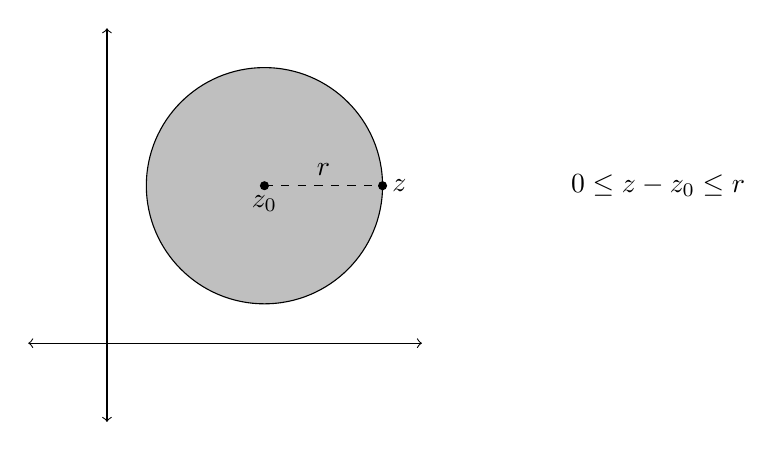
\begin{tikzpicture}
\draw [<->] (-1,0) -- (4,0);
\draw [<->] (0,-1) -- (0,4);
\draw [fill=lightgray] (2,2) circle [radius=1.5];
\draw [fill=black] (2,2) circle [radius=0.05];
\draw [fill=black] (3.5,2) circle [radius=0.05];
\draw [dashed] (2,2) -- (3.5,2);
\node [below] at (2,2) {$z_0$};
\node [right] at (3.5,2) {$z$};
\node [above] at (2.75,2) {$r$};
\node at (7,2) {$0\le\abs{z-z_0}\le r$};
\end{tikzpicture}
\end{figure}

\item{Open Disk}
\begin{figure}[h]
\setlength{\leftskip}{0.5in}
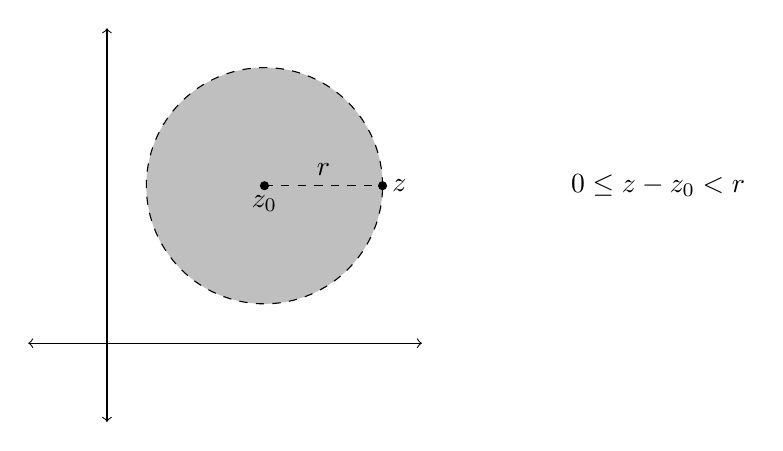
\begin{tikzpicture}
\draw [<->] (-1,0) -- (4,0);
\draw [<->] (0,-1) -- (0,4);
\draw [dashed,fill=lightgray] (2,2) circle [radius=1.5];
\draw [fill=black] (2,2) circle [radius=0.05];
\draw [fill=black] (3.5,2) circle [radius=0.05];
\draw [dashed] (2,2) -- (3.5,2);
\node [below] at (2,2) {$z_0$};
\node [right] at (3.5,2) {$z$};
\node [above] at (2.75,2) {$r$};
\node at (7,2) {$0\le\abs{z-z_0}<r$};
\end{tikzpicture}
\end{figure}

\begin{example}
Describe: $\abs{z-1}\le2\abs{z+1}$
\begin{eqnarray*}
\abs{z-1}^2 &\le& 4\abs{z+1}^2 \\
\abs{z}^2+1-2Re(z) &\le& 4(\abs{z}^2+1+2Re(z)) \\
3\abs{z}^2+3+10Re(z) &\ge& 0 \\
\abs{z}^2+1+\frac{10}{3}Re(z) &\ge& 0 \\
\abs{z}^2+\frac{10}{3}Re(z) &\ge& -1 \\
\abs{z}^2+\frac{25}{9}+\frac{10}{3}Re(z) &\ge& -1+\frac{25}{9} \\
\abs{z+\frac{5}{3}}^2 &\ge& \frac{16}{9} \\
\abs{z+\frac{5}{3}} &\ge& \frac{4}{3} \\
\end{eqnarray*}
This is the exterior of the open disk with center $z_0=\frac{5}{3}$ and
radius $r=\frac{4}{3}$.
\begin{figure}[h]
\setlength{\leftskip}{0.5in}
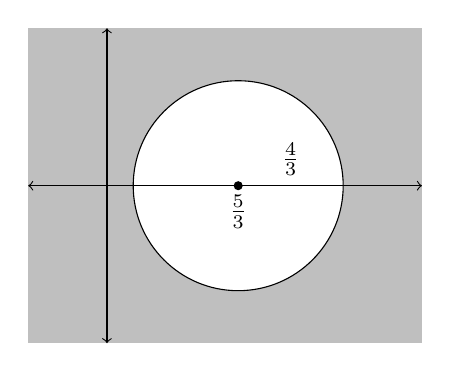
\begin{tikzpicture}
\fill [lightgray] (-1,-2) rectangle (4,2);
\draw [fill=white] (5/3,0) circle [radius=4/3];
\draw [<->] (-1,0) -- (4,0);
\draw [<->] (0,-2) -- (0,2);
\draw [fill=black] (5/3,0) circle [radius=0.05];
\node [below] at (5/3,0) {$\frac{5}{3}$};
\node [above] at (7/3,0) {$\frac{4}{3}$};
\end{tikzpicture}
\end{figure}
\end{example}

\newpage

\item{Punctured Disk}
\begin{figure}[h]
\setlength{\leftskip}{0.5in}
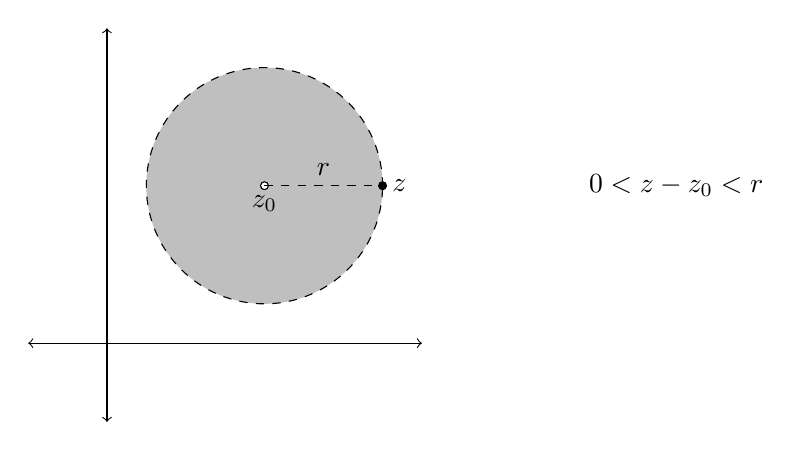
\begin{tikzpicture}
\draw [<->] (-1,0) -- (4,0);
\draw [<->] (0,-1) -- (0,4);
\draw [dashed,fill=lightgray] (2,2) circle [radius=1.5];
\draw [fill=white] (2,2) circle [radius=0.05];
\draw [fill=black] (3.5,2) circle [radius=0.05];
\draw [dashed] (2,2) -- (3.5,2);
\node [below] at (2,2) {$z_0$};
\node [right] at (3.5,2) {$z$};
\node [above] at (2.75,2) {$r$};
\node [right] at (6,2) {$0<\abs{z-z_0}<r$};
\end{tikzpicture}
\end{figure}

\item{Ellipse}
\begin{figure}[h]
\setlength{\leftskip}{0.5in}
\begin{tikzpicture}
\draw [<->] (-3,0) -- (3,0);
\draw [<->] (0,-2) -- (0,2);
\draw [fill=black] (-1.5,0) circle [radius=0.05];
\draw [fill=black] (1.5,0) circle [radius=0.05];
\draw [fill=black] (1,0.866,0) circle [radius=0.05];
\draw (0,0) ellipse (2 and 1);
\draw [dashed] (-1.5,0) -- (1,0.866);
\draw [dashed] (1.5,0) -- (1,0.866);
\node [below] at (-1.5,0) {$-a$};
\node [below] at (1.5,0) {$a$};
\node [above right] at (1,0.866) {$z$};
\node [right] at (5,0) {$\abs{z+a}+\abs{z-a}=\ell$};
\end{tikzpicture}
\end{figure}

\item{Hyperbola}
\begin{figure}[h]
\setlength{\leftskip}{0.5in}
\begin{tikzpicture}
\draw [<->] (-3,0) -- (3,0);
\draw [<->] (0,-3) -- (0,3);
\draw [fill=black] (-1.5,0) circle [radius=0.05];
\draw [fill=black] (1.5,0) circle [radius=0.05];
\draw [fill=black] (2,1.732,0) circle [radius=0.05];
\draw [dashed] (-1.5,0) -- (2,1.732);
\draw [dashed] (1.5,0) -- (2,1.732);
\node [below] at (-1.5,0) {$-a$};
\node [below] at (1.5,0) {$a$};
\node [above left] at (2,1.732) {$z$};
\draw [domain=1:3] plot (\x,{sqrt((\x)^2-1)});
\draw [domain=1:3] plot (\x,{-sqrt((\x)^2-1)});
\draw [domain=-1:-3] plot (\x,{sqrt((\x)^2-1)});
\draw [domain=-1:-3] plot (\x,{-sqrt((\x)^2-1)});
\node [right] at (5,0) {$\abs{\abs{z+a}-\abs{z-a}}=\ell$};
\end{tikzpicture}
\end{figure}

\newpage

\begin{example}
Consider the hyperbola: $x^2-y^2=1$
\begin{eqnarray*}
x^2-y^2 &=& 1 \\
Re(z)^2-Im(z)^2 &=& 1 \\
\left(\frac{z+\conj{z}}{2}\right)^2-
    \left(\frac{z-\conj{z}}{2i}\right)^2 &=& 1 \\
(z+\conj{z})^2+(z-\conj{z})^2 &=& 4 \\
(z^2+\conj{z}^2+2z\conj{z})+(z^2+\conj{z}^2-2z\conj{z}) &=& 4 \\
2z^2+2\conj{z}^2 &=& 4 \\
z^2+\conj{z}^2 &=& 2 \\
\end{eqnarray*}
\end{example}
\end{enumerate}
\end{document}
